\documentclass[a4paper,11pt,oneside]{book}
\usepackage{listings}
\usepackage[utf8]{inputenc}
\usepackage[spanish,es-tabla]{babel}

%\usepackage[style=list,number=none]{glossary}
\usepackage{titlesec}
%\usepackage{pailatino}

\decimalpoint
\usepackage{dcolumn}
\newcolumntype{.}{D{.}{\esperiod}{-1}}
\makeatletter
\addto\shorthandsspanish{\let\esperiod\es@period@code}
\makeatother

%\RequirePackage{verbatim}
%\RequirePackage[Glenn]{fncychap}
\usepackage{fancyhdr}
\usepackage{graphicx}
\usepackage{afterpage}
\usepackage{longtable}
\usepackage[pdfborder={000}]{hyperref} %referencia

% ********************************************************************
% Información reutilizable
% ********************************************************************
\newcommand{\asunto}{Trabajo de Fin de Grado}
\newcommand{\titulo}{Un portal de transparencia para datos libres}
\newcommand{\tituloEng}{A transparency portal for open data}
\newcommand{\titulacion}{Grado en Ingeniería Informática}
\newcommand{\autor}{Germán Martínez Maldonado}
\newcommand{\email}{germaaan@gmail.com}
\newcommand{\tutor}{Juan Julián Merelo Guervós}
\newcommand{\escuela}{Escuela Técnica Superior de Ingenierías Informática y de Telecomunicación}
\newcommand{\universidad}{Universidad de Granada}
\newcommand{\ciudad}{Granada}
\newcommand{\version}{Version 0.1}

\hypersetup{
pdfauthor = {\autor\ (\email)},
pdftitle = {\titulo},
pdfsubject = {\asunto},
pdfkeywords = {software libre, transparencia, datos abiertos, sistema de control de versiones, aprovisionamiento, tests, 
integración continua, despliegue automático},
pdfcreator = {LaTeX con el paquete texlive},
pdfproducer = {pdflatex}
}

%\hyphenation{}

\usepackage{url}
\usepackage{colortbl,longtable}
\usepackage[stable]{footmisc}
%\usepackage{index}

%\makeindex
%\usepackage[style=long,cols=2,border=plain,toc=true,number=none]{glossary}
%\makeglossary

% Redefinición de comandos
%\renewcommand{\indexname}{Índice alfabético}
%\renewcommand{\glossaryname}{Glosario}

\pagestyle{fancy}
\fancyhf{}
\fancyhead[LO]{\leftmark}
\fancyhead[RE]{\rightmark}
\fancyhead[RO,LE]{\textbf{\thepage}}
\renewcommand{\chaptermark}[1]{\markboth{\textbf{#1}}{}}
\renewcommand{\sectionmark}[1]{\markright{\textbf{\thesection. #1}}}

\setlength{\headheight}{1.5\headheight}

\newcommand{\HRule}{\rule{\linewidth}{0.5mm}}
%Definimos los tipos ejemplo y definición podremos usar estos tipos
\newtheorem{ejemplo}{Ejemplo}[chapter]
\newtheorem{definicion}{Definición}[chapter]

\definecolor{gray97}{gray}{.97}
\definecolor{gray75}{gray}{.75}
\definecolor{gray45}{gray}{.45}
\definecolor{gray30}{gray}{.94}

\lstset{
  frame=Ltb,
  framerule=0.5pt,
  aboveskip=0.5cm,
  framextopmargin=3pt,
  framexbottommargin=3pt,
  framexleftmargin=0.1cm,
  framesep=0pt,
  rulesep=.4pt,
  backgroundcolor=\color{gray97},
  rulesepcolor=\color{black},
  %
  stringstyle=\ttfamily,
  showstringspaces = false,
  basicstyle=\scriptsize\ttfamily,
  commentstyle=\color{gray45},
  keywordstyle=\bfseries,
  %
  numbers=left,
  numbersep=6pt,
  numberstyle=\tiny,
  numberfirstline = false,
  breaklines=true,
}
 
% Minimizar fragmentado de listados
\lstnewenvironment{listing}[1][]
  {\lstset{#1}\pagebreak[0]}{\pagebreak[0]}

% http://tex.stackexchange.com/questions/89574/language-option-supported-in-listings
\lstdefinelanguage{JavaScript}{
  keywords={typeof,new,true,false,catch,function,return,null,catch,switch,var,if,in,while,do,else,case,break},
  keywordstyle=\color{blue}\bfseries,
  ndkeywords={class,export,boolean,throw,implements,import,this},
  ndkeywordstyle=\color{darkgray}\bfseries,
  identifierstyle=\color{black},
  sensitive=false,
  comment=[l]{//},
  morecomment=[s]{/*}{*/},
  commentstyle=\color{purple}\ttfamily,
  stringstyle=\color{red}\ttfamily,
  morestring=[b]',
  morestring=[b]"
}

\lstdefinestyle{Consola}{
  basicstyle=\scriptsize\bf\ttfamily,
  backgroundcolor=\color{gray30},
  frame=single,
  numbers=none
}

\newcommand{\bigrule}{\titlerule[0.5mm]}

% Para que las páginas en blanco no tengan cabecera
\makeatletter
\def\clearpage{%
  \ifvmode
    \ifnum \@dbltopnum =\m@ne
      \ifdim \pagetotal <\topskip
        \hbox{}
      \fi
    \fi
  \fi
  \newpage
  \thispagestyle{empty}
  \write\m@ne{}
  \vbox{}
  \penalty -\@Mi
}
\makeatother

\usepackage{pdfpages}

\begin{document}
\begin{titlepage}
 
 
\newlength{\centeroffset}
\setlength{\centeroffset}{-0.5\oddsidemargin}
\addtolength{\centeroffset}{0.5\evensidemargin}
\thispagestyle{empty}

\noindent\hspace*{\centeroffset}\begin{minipage}{\textwidth}

\centering
\includegraphics[width=0.9\textwidth]{imagenes/logo_ugr.jpg}\\[1.4cm]

\textsc{ \Large TRABAJO FIN DE GRADO\\[0.2cm]}
\textsc{ GRADO INGENIERÍA EN INGENIERIA INFORMATICA}\\[1cm]
% Upper part of the page
% 
% Title
{\Huge\bfseries Un portal de transparencia para datos libres\\}
\noindent\rule[-1ex]{\textwidth}{3pt}\\[3.5ex]
%{\large\bfseries Subtitulo del Proyecto}
\end{minipage}

\vspace{2.5cm}
\noindent\hspace*{\centeroffset}\begin{minipage}{\textwidth}
\centering

\textbf{Autor}\\ {Germán Martínez Maldonado}\\[2.5ex]
\textbf{Tutor}\\ {Juan Julián Merelo Guervós}\\[2cm]
\includegraphics[width=0.3\textwidth]{imagenes/etsiit_logo.png}\\[0.1cm]
\textsc{Escuela Técnica Superior de Ingenierías Informática y de Telecomunicación}\\
\textsc{---}\\
Granada, Julio de 2015
\end{minipage}
%\addtolength{\textwidth}{\centeroffset}
%\vspace{\stretch{2}}
\end{titlepage}



\chapter*{}
%\thispagestyle{empty}
%\cleardoublepage

%\thispagestyle{empty}

\cleardoublepage
\thispagestyle{empty}

\begin{center}
{\large\bfseries \titulo}\\
\end{center}
\begin{center}
\autor\\
\end{center}

%\vspace{0.7cm}
\noindent{\textbf{Palabras clave}: palabra\_clave1, palabra\_clave2, palabra\_clave3, palabra\_clave4, palabra\_clave5}\\

\vspace{0.7cm}
\noindent{\textbf{Resumen}}\\

Poner aquí el resumen.
\cleardoublepage

\thispagestyle{empty}

\begin{center}
{\large\bfseries \tituloEng}\\
\end{center}
\begin{center}
\autor\\
\end{center}

%\vspace{0.7cm}
\noindent{\textbf{Keywords}: keyword1, keyword2, keyword3, keyword4, keyword5}\\

\vspace{0.7cm}
\noindent{\textbf{Abstract}}\\

Write here the abstract in English.

\chapter*{}
\thispagestyle{empty}

\noindent\rule[-1ex]{\textwidth}{2pt}\\[4.5ex]

Yo, \textbf{\autor}, alumno de la titulación \titulacion de la \textbf{\escuela\ de la \universidad}, con DNI XXXXXXXXX, 
autorizo la ubicación de la siguiente copia de mi Trabajo Fin de Grado en la biblioteca del centro para que pueda ser
consultada por las personas que lo deseen.

\vspace{6cm}

\noindent Fdo: \autor

\vspace{2cm}

\begin{flushright}
\ciudad, a \today
\end{flushright}

\chapter*{}
\thispagestyle{empty}

\noindent\rule[-1ex]{\textwidth}{2pt}\\[4.5ex]

D. \textbf{\tutor}, Profesor del Área de XXXX del Departamento de Arquitectura y Tecnología de Computadores de la \universidad.

\vspace{0.5cm}

\vspace{0.5cm}

\textbf{Informa:}

\vspace{0.5cm}

Que el presente trabajo, titulado \textit{\textbf{\titulo}}, ha sido realizado bajo su supervisión por \textbf{\autor}, y 
autorizo la defensa de dicho trabajo ante el tribunal que corresponda.

\vspace{0.5cm}

Y para que conste, expide y firma el presente informe en \ciudad\ a \today.

\vspace{1cm}

\textbf{El tutor:}

\vspace{5cm}

\noindent \textbf{\tutor}

\chapter*{Agradecimientos}
\thispagestyle{empty}

\vspace{1cm}

Poner aquí agradecimientos...



%\frontmatter
\tableofcontents
%\listoffigures
%\listoftables
%
%\mainmatter
%\setlength{\parskip}{5pt}

\newpage
\thispagestyle{empty}
\
\chapter{Introducción}

En la actualidad, nuestro país al igual que muchos otros se rige por lo que se conoce como \textbf{``democracia''}. Si buscamos
el significado de esta palabra, encontraremos que su definición es: 

\begin{quote}Sistema político que defiende la soberanía del pueblo y el derecho del pueblo a elegir y controlar a sus 
gobernantes.
\newline(\url{http://www.oxforddictionaries.com/es/definicion/espanol/democracia})
\end{quote}

Aunque \textit{``el derecho del pueblo a elegir''} es lo importante, para que esa elección pueda ser coherente, primero será el propio
pueblo el que deberá tener la obligación a conocer lo que elige, y la única forma de conocer lo que se elige es a través de la
transparencia. Por este motivo, el pueblo debe exigir transparencia en el funcionamiento de las instituciones públicas, y esas
instituciones públicas siempre no tengan nada que esconder debería facilitar de buena fe (y no porque haya una ley que les 
obligue) todo la información que el ciudadano le requiera.

\bigskip
Estas inquietudes fueron las que hicieron en un primer momento que se comenzara con el desarrollo del Portal de Transparencia
de la Universidad de Granada a principios del año pasado, cuyo desarrollo le fue encargado a la Oficina de Software Libre de la propia universidad y 
aproximadamente a los 7 meses de comenzar su desarrollo fue presentada una primera versión.

\bigskip
En febrero de este año entré como becario en la Oficina de Software Libre y me integré en el equipo de desarrollo del portal,
siendo mis mayores contribuciones cambiar el origen de datos de la página para eliminar un error que se producia recurrentemente
durante la navegación por el parte, y además, implantar una metodología de desarrollo DevOps.

\newpage
Una metodología de desarrollo DevOps consiste inicialmente en no hacer distinción entre el desarrollo del software y la
administración del mismo, todo estará comunicado para que sea posible realizar entregas del software de forma frecuente 
asegurándose de que esas mismas entregas continuas no sea el origen de fallos futuros. La forma de asegurarse de que esos
fallos no se producirán es dividir todo el desarrollo en fases que tengan que realizarse secuencialmente, controlando a cada
fase que no se produzcan errores en la misma; como una cadena de montaje en la que podemos estar seguro de que el producto
que llega al final está en perfectas condiciones, porque en caso contrario hubiera sido retirado durante el proceso.

\bigskip
En este proyecto, hemos considerado que las fases que nos permitirían asegurarnos que el producto que sale de la cadena de 
montaje en perfectas condiciones sean los test unitarios, la integración continua y el despliegue automático, todo esto apoyado
en un sistema de control de versiones y una plataforma de desarrollo colaborativo abierto. Además, también se usará
aprovisionamiento para facilitar la portabilidad del portal de una infraestructura a otra distinta. Se ahondará en el 
funcionamiento de todos estos conceptos en el capítulo 5 (Implementación), donde se explicará detenidamente como han sido 
integrados en el proyecto.
\chapter{Planificación}

\section{Fases y entregas}

\subsection{Fases}

Como este va a ser un proyecto que ya cuenta con un trabajo previo realizado, la fase inicial de gestión va a ser muy breve
porque se parte de que ya se han realizado varias reuniones y el proyecto está parcialmente funcionando, por lo que no se parte
de cero, es una ampliación de un proyecto inicial.

\begin{itemize}
  \item \textbf{Fase 0:} Gestión del proyecto
  \item \textbf{Fase 1:} Análisis del entorno
  \item \textbf{Fase 2:} Desarrollo del Documento de Objetivos del Proyecto
  \item \textbf{Fase 3:} Desarrollo técnico
\end{itemize}

\subsection{Lista de entregas}

Se harán una serie de breves informes sobre el contenido de cada una de las fases de planificación del proyecto.

\begin{itemize}
  \item \textbf{Fase 0:} Gestión del proyecto
  \begin{itemize}
    \item Descripción: Se realizarán reuniones para concretar los objetivos del proyecto y el desarrollo necesario para 
    cumplirlo.
    \item Tipo: informe.
  \end{itemize}
  \item \textbf{Fase 1:} Análisis del entorno
  \begin{itemize}
    \item Descripción: Se establecen los criterios de elección de las herramientas a utilizar.
    \item Tipo: informe.
  \end{itemize}
  \item \textbf{Fase 2:} Desarrollo del Documento de Objetivos del Proyecto
  \begin{itemize}
    \item Descripción: Se desarrolla un documento que recoja los objetivos a cumplir en el proyecto, así como diferentes
    aspectos del proyecto que habrá que tener en cuando para su puesta en desarrollo.
    \item Tipo: informe.
  \end{itemize}
  \item \textbf{Fase 3:} Desarrollo técnico
  \begin{itemize}
    \item Descripción: Implementación del software necesario para cumplir los objetivos, pasando por sus diferentes fases: 
    análisis, diseño, implementación, pruebas. También se realizará una documentación explicativa sobre funcionamiento del 
    mismo.
    \item Tipo: informe.
  \end{itemize}
\end{itemize}

\section{Estructura de Descomposición del Trabajo}

El diagrama de Estructura de Descomposición del Trabajo (figura 2.1) es una descomposición jerárquica de las diferentes fases y 
entregas en las que está planificado el proyecto.

\begin{figure}[h]
\caption{Diagramas de casos de uso}
\centering
\includegraphics[width=1.1\textwidth]{imagenes/edt.png}
\end{figure}

\section{Actividades y tiempo}

\section{Dependencias entre tareas}

\section{Asignación de recursos}

\section{Diagrama de Gantt}

\section{Análisis de costes}

\input{capitulos/03_EspecificacionRequisitos}
%
%\chapter{Análisis}

\section{Análisis de requisitos}

Todo software se desarrolla para cubrir una necesidad, por lo que en este apartado vamos a describir los requisitos que se estiman necesarios para cubrir los objetivos propuestos.

\subsection{Descripción de los actores}

Los actores implicados serán dos: el \textbf{desarrollador} y el \textbf{usuario}.

\bigskip
El \textbf{desarrollador} será el encargado de solucionar los problemas de visualización de los datos en el portal, además de portar el desarrollo actual del portal a un entorno de desarrollo continuo. También asumirá la administración del portal ya que este tipo de rol está muy integrado con las labores de despliegue en el desarrollo continuo.

\bigskip
El \textbf{usuario} de la aplicación será cualquier persona que tenga interés por conocer datos internos de la \textbf{Universidad de Granada} fácilmente. El usuario no pertenece a ningún público objetivo concreto, por lo que no se tiene que considerar que tenga una experiencia previa en navegador por sitios web.

\bigskip
Los dos tipos de actores descritos son la generalización de todo los tipos de personas que usarían el portal, sin embargo, podríamos hacer un análisis más extenso si nos basáramos en una metodología orientada al usuario como \textbf{persona}. Una persona sería la representación de usuarios que comparten objetivos y a los que se espera comportamientos similares. Un par de ejemplos:

\newpage
\begin{itemize}
	\item Alguien de la propia \textbf{Universidad de Granada} y de otra universidad que accedan al portal, ambos encajarían dentro del actor \textbf{usuario}, sin embargo eso no quiere decir que el objetivo de ambos sea el mismo, los usuarios de la propia universidad pueden querer consultar datos únicamente y los de otra universidad puede que estén más interesados en ver la estructura de las páginas del portal.
	\item Alguien que quiera hacer una despliegue de la aplicación, puede que no quiere hacerlo para una universidad sino para un ayuntamiento, volvemos a estar en el mismo caso, ambos entrarían en el tipo de actor \textbf{desarrollador}, pero sus intenciones e interés son muy distintos entre sí.
\end{itemize}

\subsection{Requisitos funcionales}

Los requisitos funcionales son las características que tiene que implementar el sistema para cubrir todas las necesidades de los distintos usuarios.

\bigskip
Al usuario lo único que le interesa es ver una página web estática con la información que desea 
consultar, para ello el desarrollador deberá hacer que sea posible que se generen siempre las tablas con los elementos de información. 

\bigskip
Por otra parte, el desarrollador quiere integrar el sistema en un desarrollo continuo, por lo que añadirá tests unitarios, test de cobertura, integración continua, despliegue automático y provisionamiento con tal fin.

\begin{itemize}
  \item \textbf{RF-1.} Administración portal:
    \begin{itemize}
    \item \textbf{RF-1.1.} Automatizar inicio del servidor del portal.
    \end{itemize}
\end{itemize}

\begin{itemize}
  \item \textbf{RF-2.} Acceso información:
    \begin{itemize}
    \item \textbf{RF-2.1.} Consultar información de \textit{Administración}.
    \item \textbf{RF-2.1.} Consultar información de \textit{Docencia}.
    \item \textbf{RF-2.1.} Consultar información de \textit{Gestión e Investigación}.
    \item \textbf{RF-2.1.} Consultar información de \textit{Normativa Legal}.
    \end{itemize}
\end{itemize}

\begin{itemize}
  \item \textbf{RF-3.} Pruebas de software:
  \begin{itemize}
    \item \textbf{RF-3.1.} Realizar tests unitarios.
    \item \textbf{RF-3.2.} Realizar test de cobertura.
    \item \textbf{RF-3.2.} Usar integración continua.
    \end{itemize}
\end{itemize}

\begin{itemize}
  \item \textbf{RF-4.} Configuración automática:
  \begin{itemize}
    \item \textbf{RF-4.1.} Usar despliegue automático.
    \item \textbf{RF-4.2.} Usar provisionamiento.
    \end{itemize}
\end{itemize}

\subsection{Requisitos no funcionales}

Los requisitos no funcionales son las características propias del desarrollo, pero que no tienen que estar relacionadas con su funcionalidad.

\begin{itemize}
  \item \textbf{RN-1.} Toda la programación del portal se hará en {\tt Node.js} y los módulos que se usen deben ser instalables a través de su gestor de paquetes {\tt NPM}.
  \item \textbf{RN-2.} El portal se iniciará y se detendrá mediante scripts lanzados con {\tt NPM}.
  \item \textbf{RN-3.} Para iniciar la ejecución del portal es necesario que reciba el puerto de escucha del servidor y la dirección de acceso.
  \item \textbf{RN-4.} Todos los módulos se ejecutarán desde scripts lanzamos con {\tt NPM}.
  \item \textbf{RN-5.} Los tests unitarios se realizarán en base a comportamientos esperados y valores de estados.
  recibidos como contestación a las peticiones que se realicen al portal.
  \item \textbf{RN-6.} Los tests unitarios tienen que recibir las páginas del portal para ejecutarse.
  \item \textbf{RN-7.} El test de cobertura tiene que tener una automatización integrable con los tests unitarios. 
  \item \textbf{RN-8.} La integración continua se ejecutará automáticamente con cada cambio que se haga en la programación del portal.
  \item \textbf{RN-9.} El despliegue automático se realizará mediante conexiones {\tt SSH}.
  \item \textbf{RN-10.} Tanto para el despliegue automático como para el provisionamiento es necesario indicar el usuario que lo realiza y el destino en el que se realiza.
\end{itemize}

\subsection{Requisitos de información}

Los requisitos de información se refieren a la información que es necesaria almacenar en el sistema. La única información relevante que se va a almacenar son los datos descriptivos y de enlace de cada uno de los elementos del portal {\tt OpenData UGR} que se van a mostrar en {\tt UGR Transparente}.

\begin{itemize}
  \item \textbf{RI-1.} Datos abiertos.
  \begin{itemize}
    \item Información sobre cada uno de los elementos que se van a mostrar en el portal de transparencia como datos abiertos.
    \item Contenido: nombre, categoría, conjunto de datos, enlace a {\tt OpenData UGR}, enlace al recurso.
  \end{itemize}
\end{itemize}

\section{Modelos de casos de uso}

Aunque ya se ha indicado que la parte funcional ya se encuentra implementada de forma previa a este proyecto, se van a incluir unos modelos de caso de uso simples para dar un visión más clara del funcionamiento general del portal {\tt UGR Transparente}.

\subsection{Descripción básica de actores}

\begin{itemize}
  \item \textbf{Ac-1.} Desarrollador.
  \begin{itemize}
   \item Descripción: Encargado del desarrollo y administración del portal.
   \item Características: Su trabajo está en el lado del servidor que genera la página, nunca trabaja desde el lado del cliente.
   \item Relaciones: Ninguna.
   \item Atributos: Ninguno.
   \item Comentarios: Es el encargado de que la información se muestre en el portal y de añadir funcionalidades al portal.
  \end{itemize}
  
  \item \textbf{Ac-2.} Usuario.
  \begin{itemize}
   \item Descripción: Persona que usa el portal para consultar datos.
   \item Características: Es el usuario común que accederá a la página.
   \item Relaciones: Ninguna.
   \item Atributos: Ninguno.
   \item Comentarios: El usuario no es necesario que tenga ningún conocimiento previo al uso del portal, simplemente accederá y consultará los datos que sean de su interés.
  \end{itemize}
\end{itemize}

\subsection{Descripción casos de uso}

\begin{itemize}
  \item \textbf{CU-1.} Inicio automático del servidor del portal.
  \begin{itemize}
    \item Actores: Desarrollador.
    \item Tipo: Primario, esencial.
    \item Referencias:
    \item Precondición: El servidor esté detenido.
    \item Postcondición: El portal será accesible públicamente.
    \item Autor: \autor.
    \item Versión: 1.0.
    \item Propósito: Iniciar el servidor del portal {\tt UGR Transparente}.
    \item Resumen: Cuando se ejecuta el script de inicio de la aplicación, arranca el servidor y el portal será accesible desde Internet.
    \begin{table}[!ht]
      \begin{center}
	\begin{tabular}{|l|l|l|l|}
	  \hline
	  \multicolumn{4}{|c|}{{\bf Curso normal}}
	  \\ \hline
	  \multicolumn{2}{|c|}{{\bf Actor}} & \multicolumn{2}{c|}{{\bf Sistema}}
	  \\ \hline
	  {\it 1} & 
	  \begin{tabular}[c]{@{}l@{}}
	    Desarrollador: da orden de\\
	    que se inicie el servidor\\
	    del portal.
	  \end{tabular} &
	  &
	  \\ \hline
	  &
	  &
	  {\it 2a} &
	  \begin{tabular}[c]{@{}l@{}}
	    Comprueba que el servidor\\
	    está detenido y lo inicia\\
	    para que el portal esté\\
	    operativo.
	  \end{tabular}
	  \\ \hline
	\end{tabular}
	\caption{Curso normal de CU-1. Inicio automático del servidor del portal}
	\label{table:cn_cu_1}
      \end{center}
    \end{table}
    \begin{table}[!ht]
      \begin{center}
	\begin{tabular}{|l|l|}
	  \hline
	  \multicolumn{2}{|c|}{{\bf Curso alterno}}
	  \\ \hline
	  {\it 2b} &
	  \begin{tabular}[c]{@{}l@{}}
	    Si el servidor está funcionando, no se ejecuta el script de\\
	    inicio del servidor.
	  \end{tabular}\\
	  \hline
	\end{tabular}
	\caption{Curso alterno de CU-1. Inicio automático del servidor del portal}
	\label{table:ca_cu_1}
      \end{center}
    \end{table}
  \end{itemize}
 
  \newpage
  \item \textbf{CU-2.} Consultar información de \textit{Administración}.
  \begin{itemize}
    \item Actores: Usuario.
    \item Tipo: Primario, esencial.
    \item Referencias:
    \item Precondición: Existan archivos con los datos abiertos.
    \item Postcondición:
    \item Autor: \autor.
    \item Versión: 1.0.
    \item Propósito: El usuario consulta datos de administración en el portal {\tt UGR Transparente}.
    \item Resumen: El usuario que accede al portal de transparencia selecciona la sección de \textit{Administración} y consulta la información de sus subsecciones.
    \begin{table}[!ht]
      \begin{center}
	\begin{tabular}{|l|l|l|l|}
	  \hline
	  \multicolumn{4}{|c|}{{\bf Curso normal}}
	  \\ \hline
	  \multicolumn{2}{|c|}{{\bf Actor}} & \multicolumn{2}{c|}{{\bf Sistema}}
	  \\ \hline
	  {\it 1} & 
	  \begin{tabular}[c]{@{}l@{}}
	    Usuario: consulta la información\\
	    de \textit{Administración} publicada en el\\
	    portal.
	  \end{tabular} &
	  &
	  \\ \hline
	  &
	  &
	  {\it 2} &
	  \begin{tabular}[c]{@{}l@{}}
	    Se generan las tablas con\\
	    todos los elementos de\\
	    información de la sección\\
	    \textit{Administración}.
	  \end{tabular}
	  \\ \hline
	  &
	  &
	  {\it 3} &
	  \begin{tabular}[c]{@{}l@{}}
	    Se muestran en la página\\
	    todos las tablas generadas\\
	    con los elementos de\\
	    información.
	  \end{tabular}
	  \\ \hline
	\end{tabular}
	\caption{Curso normal de CU-2. Consultar información de Administración}
	\label{table:cn_cu_2}
      \end{center}
    \end{table}
  \end{itemize}
  
  \newpage
  \item \textbf{CU-3.} Consultar información de \textit{Docencia}.
  \begin{itemize}
    \item Actores: Usuario.
    \item Tipo: Primario, esencial.
    \item Referencias:
    \item Precondición: Existan archivos con los datos abiertos.
    \item Postcondición:
    \item Autor: \autor.
    \item Versión: 1.0.
    \item Propósito: El usuario consulta datos de administración en el portal {\tt UGR Transparente}.
    \item Resumen: El usuario que accede al portal de transparencia selecciona la sección de \textit{Docencia} y consulta la información de sus subsecciones.
    \begin{table}[!ht]
      \begin{center}
	\begin{tabular}{|l|l|l|l|}
	  \hline
	  \multicolumn{4}{|c|}{{\bf Curso normal}}
	  \\ \hline
	  \multicolumn{2}{|c|}{{\bf Actor}} & \multicolumn{2}{c|}{{\bf Sistema}}
	  \\ \hline
	  {\it 1} & 
	  \begin{tabular}[c]{@{}l@{}}
	    Usuario: consulta la información\\
	    de \textit{Docencia} publicada en el\\
	    portal.
	  \end{tabular} &
	  &
	  \\ \hline
	  &
	  &
	  {\it 2} &
	  \begin{tabular}[c]{@{}l@{}}
	    Se generan las tablas con\\
	    todos los elementos de\\
	    información de la sección\\
	    \textit{Docencia}.
	  \end{tabular}
	  \\ \hline
	  &
	  &
	  {\it 3} &
	  \begin{tabular}[c]{@{}l@{}}
	    Se muestran en la página\\
	    todos las tablas generadas\\
	    con los elementos de\\
	    información.
	  \end{tabular}
	  \\ \hline
	\end{tabular}
	\caption{Curso normal de CU-3. Consultar información de Docencia}
	\label{table:cn_cu_3}
      \end{center}
    \end{table}
  \end{itemize}
  
  \newpage
  \item \textbf{CU-4.} Consultar información de \textit{Gestión e Investigación}.
  \begin{itemize}
    \item Actores: Usuario.
    \item Tipo: Primario, esencial.
    \item Referencias:
    \item Precondición: Existan archivos con los datos abiertos.
    \item Postcondición:
    \item Autor: \autor.
    \item Versión: 1.0.
    \item Propósito: El usuario consulta datos de administración en el portal {\tt UGR Transparente}.
    \item Resumen: El usuario que accede al portal de transparencia selecciona la sección de \textit{Gestión e Investigación} y consulta la información de sus subsecciones.
    \begin{table}[!ht]
      \begin{center}
	\begin{tabular}{|l|l|l|l|}
	  \hline
	  \multicolumn{4}{|c|}{{\bf Curso normal}}
	  \\ \hline
	  \multicolumn{2}{|c|}{{\bf Actor}} & \multicolumn{2}{c|}{{\bf Sistema}}
	  \\ \hline
	  {\it 1} & 
	  \begin{tabular}[c]{@{}l@{}}
	    Usuario: consulta la información\\
	    de \textit{Gestión e Investigación} publicada\\
	    en el portal.
	  \end{tabular} &
	  &
	  \\ \hline
	  &
	  &
	  {\it 2} &
	  \begin{tabular}[c]{@{}l@{}}
	    Se generan las tablas con\\
	    todos los elementos de\\
	    información de la sección\\
	    \textit{Gestión e Investigación}.
	  \end{tabular}
	  \\ \hline
	  &
	  &
	  {\it 3} &
	  \begin{tabular}[c]{@{}l@{}}
	    Se muestran en la página\\
	    todos las tablas generadas\\
	    con los elementos de\\
	    información.
	  \end{tabular}
	  \\ \hline
	\end{tabular}
	\caption{Curso normal de CU-4. Consultar información de Gestión e Investigación}
	\label{table:cn_cu_4}
      \end{center}
    \end{table}
  \end{itemize}
  
  \newpage
  \item \textbf{CU-5.} Consultar información de \textit{Normativa Legal}.
  \begin{itemize}
    \item Actores: Usuario.
    \item Tipo: Primario, esencial.
    \item Referencias:
    \item Precondición: Existan archivos con los datos abiertos.
    \item Postcondición:
    \item Autor: \autor.
    \item Versión: 1.0.
    \item Propósito: El usuario consulta datos de administración en el portal {\tt UGR Transparente}.
    \item Resumen: El usuario que accede al portal de transparencia selecciona la sección de \textit{Normativa Legal} y consulta la información de sus subsecciones.
    \begin{table}[!ht]
      \begin{center}
	\begin{tabular}{|l|l|l|l|}
	  \hline
	  \multicolumn{4}{|c|}{{\bf Curso normal}}
	  \\ \hline
	  \multicolumn{2}{|c|}{{\bf Actor}} & \multicolumn{2}{c|}{{\bf Sistema}}
	  \\ \hline
	  {\it 1} & 
	  \begin{tabular}[c]{@{}l@{}}
	    Usuario: consulta la información\\
	    de \textit{Normativa Legal} publicada en el\\
	    portal.
	  \end{tabular} &
	  &
	  \\ \hline
	  &
	  &
	  {\it 2} &
	  \begin{tabular}[c]{@{}l@{}}
	    Se generan las tablas con\\
	    todos los elementos de\\
	    información de la sección\\
	    \textit{Normativa Legal}.
	  \end{tabular}
	  \\ \hline
	  &
	  &
	  {\it 3} &
	  \begin{tabular}[c]{@{}l@{}}
	    Se muestran en la página\\
	    todos las tablas generadas\\
	    con los elementos de\\
	    información.
	  \end{tabular}
	  \\ \hline
	\end{tabular}
	\caption{Curso normal de CU-5. Consultar información de Normativa Legal}
	\label{table:cn_cu_5}
      \end{center}
    \end{table}
  \end{itemize}
 
  \newpage
  \item \textbf{CU-6.} Realizar tests unitarios.
  \begin{itemize}
    \item Actores: Desarrollador.
    \item Tipo: Primario, esencial.
    \item Referencias:
    \item Precondición: Existan tests unitarios.
    \item Postcondición: 
    \item Autor: \autor.
    \item Versión: 1.0.
    \item Propósito: Realizar tests unitarios para comprobar las funcionalidades de la aplicación.
    \item Resumen: Cada vez que se añadan nuevas páginas o funcionalidades al portal, se comprueba que funcionan correctamente.
    \begin{table}[!ht]
      \begin{center}
	\begin{tabular}{|l|l|l|l|}
	  \hline
	  \multicolumn{4}{|c|}{{\bf Curso normal}}
	  \\ \hline
	  \multicolumn{2}{|c|}{{\bf Actor}} & \multicolumn{2}{c|}{{\bf Sistema}}
	  \\ \hline
	  {\it 1} & 
	  \begin{tabular}[c]{@{}l@{}}
	    Desarrollador: da orden de\\
	    ejecutar los tests unitarios.
	  \end{tabular} &
	  &
	  \\ \hline
	  &
	  &
	  {\it 2a} &
	  \begin{tabular}[c]{@{}l@{}}
	    Comprueba que hay tests\\
	    unitarios y los ejecuta.\\
	  \end{tabular}
	  \\ \hline
	\end{tabular}
	\caption{Curso normal de CU-6. Realizar tests unitarios}
	\label{table:cn_cu_6}
      \end{center}
    \end{table}
    \begin{table}[!ht]
      \begin{center}
	\begin{tabular}{|l|l|}
	  \hline
	  \multicolumn{2}{|c|}{{\bf Curso alterno}}
	  \\ \hline
	  {\it 2b} &
	  \begin{tabular}[c]{@{}l@{}}
	    Si no hay tests unitarios creados, el sistema no hace nada.
	  \end{tabular}\\
	  \hline
	\end{tabular}
	\caption{Curso alterno de CU-6. Realizar tests unitarios}
	\label{table:ca_cu_6}
      \end{center}
    \end{table}
  \end{itemize}
 
  \newpage
  \item \textbf{CU-7.} Realizar tests de cobertura.
  \begin{itemize}
    \item Actores: Desarrollador.
    \item Tipo: Primario, esencial.
    \item Referencias: (CU-6.) Realizar tests unitarios.
    \item Precondición: Existan tests unitarios.
    \item Postcondición: 
    \item Autor: \autor.
    \item Versión: 1.0.
    \item Propósito: Realizar test de cobertura para comprobar calidad de los tests unitarios.
    \item Resumen: Para comprobar si los tests unitarios cumplen correctamente con su función se analiza el porcentaje del código que está cubierto por los mismos.
    \begin{table}[!ht]
      \begin{center}
	\begin{tabular}{|l|l|l|l|}
	  \hline
	  \multicolumn{4}{|c|}{{\bf Curso normal}}
	  \\ \hline
	  \multicolumn{2}{|c|}{{\bf Actor}} & \multicolumn{2}{c|}{{\bf Sistema}}
	  \\ \hline
	  {\it 1} & 
	  \begin{tabular}[c]{@{}l@{}}
	    Desarrollador: da orden de\\
	    ejecutar test de cobertura.
	  \end{tabular} &
	  &
	  \\ \hline
	  &
	  &
	  {\it 2a} &
	  \begin{tabular}[c]{@{}l@{}}
	    Comprueba que hay tests\\
	    unitarios y los ejecuta.\\
	  \end{tabular}
	  \\ \hline
	  &
	  &
	  {\it 3} &
	  \begin{tabular}[c]{@{}l@{}}
	    Se ejecuta el test de \\
	    cobertura en base a los\\
	    tests unitarios ejecutados.
	  \end{tabular}
	  \\ \hline
	\end{tabular}
	\caption{Curso normal de CU-7. Realizar test de cobertura}
	\label{table:cn_cu_7}
      \end{center}
    \end{table}
    \begin{table}[!ht]
      \begin{center}
	\begin{tabular}{|l|l|}
	  \hline
	  \multicolumn{2}{|c|}{{\bf Curso alterno}}
	  \\ \hline
	  {\it 2b} &
	  \begin{tabular}[c]{@{}l@{}}
	    Si no hay tests unitarios creados, el sistema no hace nada.
	  \end{tabular}\\
	  \hline
	\end{tabular}
	\caption{Curso alterno de CU-7. Realizar test de cobertura}
	\label{table:ca_cu_7}
      \end{center}
    \end{table}
  \end{itemize}
 
  \newpage
  \item \textbf{CU-8.} Usar integración continua.
  \begin{itemize}
    \item Actores: Desarrollador.
    \item Tipo: Primario, esencial.
    \item Referencias: (CU-5.) Realizar tests unitarios.
    \item Precondición: Existan test unitarios.
    \item Postcondición: Se genera un informe con el resultado de los tests unitarios.
    \item Autor: \autor.
    \item Versión: 1.0.
    \item Propósito: Comprobar si los cambios en la aplicación provocan errores.
    \item Resumen: Cuando se efectúan cambios en la aplicación automáticamente se ejecutan los tests unitarios para comprobar si los cambios introducidos provocan conflictos en la plataforma.
    \begin{table}[!ht]
      \begin{center}
	\begin{tabular}{|l|l|l|l|}
	  \hline
	  \multicolumn{4}{|c|}{{\bf Curso normal}}
	  \\ \hline
	  \multicolumn{2}{|c|}{{\bf Actor}} & \multicolumn{2}{c|}{{\bf Sistema}}
	  \\ \hline
	  {\it 1} & 
	  \begin{tabular}[c]{@{}l@{}}
	    Desarrollador: guardar\\
	    cambios en el repositorio.
	  \end{tabular} &
	  &
	  \\ \hline
	  &
	  &
	  {\it 2a} &
	  \begin{tabular}[c]{@{}l@{}}
	    Comprueba que hay tests\\
	    unitarios y comienza la\\
	    verificación de la\\
	    integración continua.
	  \end{tabular}
	  \\ \hline
	  &
	  &
	  {\it 3} &
	  \begin{tabular}[c]{@{}l@{}}
	    Ejecuta los tests unitarios\\
	    para cada entorno definido.
	  \end{tabular}
	  \\ \hline
	\end{tabular}
	\caption{Curso normal de CU-8. Usar integración continua}
	\label{table:cn_cu_8}
      \end{center}
    \end{table}
    \begin{table}[!ht]
      \begin{center}
	\begin{tabular}{|l|l|}
	  \hline
	  \multicolumn{2}{|c|}{{\bf Curso alterno}}
	  \\ \hline
	  {\it 2b} &
	  \begin{tabular}[c]{@{}l@{}}
	    Si no hay tests unitarios creados, el sistema no hace nada.
	  \end{tabular}\\
	  \hline
	\end{tabular}
	\caption{Curso alterno de CU-8. Usar integración continua}
	\label{table:ca_cu_8}
      \end{center}
    \end{table}
  \end{itemize}
 
  \newpage
  \item \textbf{CU-.9 } Usar despliegue automático.
  \begin{itemize}
    \item Actores: Desarrollador.
    \item Tipo: Primario, esencial.
    \item Referencias: (CU-1.) Iniciar plataforma.
    \item Precondición: 
    \item Postcondición: Los cambios introducidos son aplicados en la plataforma.
    \item Autor: \autor.
    \item Versión: 1.0.
    \item Propósito: Aplicar automáticamente los cambios realizados a la aplicación. 
    \item Resumen: Para no tener que acceder manualmente al servidor de la plataforma y tener que desplegar los cambios introducidos, desde el entorno de desarrollo desplegamos automáticamente los cambios en el servidor.
    \begin{table}[!ht]
      \begin{center}
	\begin{tabular}{|l|l|l|l|}
	  \hline
	  \multicolumn{4}{|c|}{{\bf Curso normal}}
	  \\ \hline
	  \multicolumn{2}{|c|}{{\bf Actor}} & \multicolumn{2}{c|}{{\bf Sistema}}
	  \\ \hline
	  {\it 1} & 
	  \begin{tabular}[c]{@{}l@{}}
	    Desarrollador: ordenar\\
	    despliegue automático.
	  \end{tabular} &
	  &
	  \\ \hline
	  &
	  &
	  {\it 2} &
	  \begin{tabular}[c]{@{}l@{}}
	    Conectar al servidor.
	  \end{tabular}
	  \\ \hline
	  &
	  &
	  {\it 3} &
	  \begin{tabular}[c]{@{}l@{}}
	    Crear copia de seguridad.
	  \end{tabular}
	  \\ \hline
	  &
	  &
	  {\it 4a} &
	  \begin{tabular}[c]{@{}l@{}}
	    Comprobar si hay cambios en\\
	    el repositorio de la\\
	    plataforma y descargarlos\\
	    en dicho caso.
	  \end{tabular}
	  \\ \hline
	  &
	  &
	  {\it 5} &
	  \begin{tabular}[c]{@{}l@{}}
	    Iniciar la plataforma con\\
	    los cambios aplicados.
	  \end{tabular}
	  \\ \hline
	\end{tabular}
	\caption{Curso normal de CU-9. Usar despliegue automático}
	\label{table:cn_cu_9}
      \end{center}
    \end{table}
    \begin{table}[!ht]
      \begin{center}
	\begin{tabular}{|l|l|}
	  \hline
	  \multicolumn{2}{|c|}{{\bf Curso alterno}}
	  \\ \hline
	  {\it 4b} &
	  \begin{tabular}[c]{@{}l@{}}
	    Si no hay cambios aplicables, se continua con el proceso.
	  \end{tabular}\\
	  \hline
	\end{tabular}
	\caption{Curso alterno de CU-9. Usar despliegue automático}
	\label{table:ca_cu_9}
      \end{center}
    \end{table}
  \end{itemize}
 
  \newpage
  \item \textbf{CU-.10} Usar provisionamiento.
  \begin{itemize}
    \item Actores: Desarrollador.
    \item Tipo: Primario, esencial.
    \item Referencias: (CU-1.) Iniciar plataforma.
    \item Precondición: 
    \item Postcondición: El portal queda instalado en la infraestructura seleccionada.
    \item Autor: \autor.
    \item Versión: 1.0.
    \item Propósito: Instalar automáticamente el portal en una infraestructura dada.
    \item Resumen: Se instalarán automáticamente todos los elementos necesarios para poner en funcionamiento el portal en cualquier infraestructura que se indique.
    \begin{table}[!ht]
      \begin{center}
	\begin{tabular}{|l|l|l|l|}
	  \hline
	  \multicolumn{4}{|c|}{{\bf Curso normal}}
	  \\ \hline
	  \multicolumn{2}{|c|}{{\bf Actor}} & \multicolumn{2}{c|}{{\bf Sistema}}
	  \\ \hline
	  {\it 1} & 
	  \begin{tabular}[c]{@{}l@{}}
	    Desarrollador: ordenar\\
	    despliegue automático.
	  \end{tabular} &
	  &
	  \\ \hline
	  &
	  &
	  {\it 2} &
	  \begin{tabular}[c]{@{}l@{}}
	    Conectar al servidor.
	  \end{tabular}
	  \\ \hline
	  &
	  &
	  {\it 3} &
	  \begin{tabular}[c]{@{}l@{}}
	    Comprobar aplicación necesaria.
	  \end{tabular}
	  \\ \hline
	  &
	  &
	  {\it 4a} &
	  \begin{tabular}[c]{@{}l@{}}
	    Se comprueba si la aplicación\\
	    necesaria está instalada,\\
	    instalándola en caso de que\\
	    no lo esté.
	  \end{tabular}
	  \\ \hline
	  &
	  &
	  {\it 5} &
	  \begin{tabular}[c]{@{}l@{}}
	    Descarga la plataforma desde\\
	    el repositorio.
	  \end{tabular}
	  \\ \hline
	  &
	  &
	  {\it 6} &
	  \begin{tabular}[c]{@{}l@{}}
	    Instalar todas las dependencias\\
	    de la plataforma.
	  \end{tabular}
	  \\ \hline
	  &
	  &
	  {\it 7} &
	  \begin{tabular}[c]{@{}l@{}}
	    Se establecen los parámetros de\\
	    acceso al portal desde Internet.
	  \end{tabular}
	  \\ \hline
	  &
	  &
	  {\it 8} &
	  \begin{tabular}[c]{@{}l@{}}
	    Con todo preparado, se inicia\\
	    la plataforma.
	  \end{tabular}
	  \\ \hline
	\end{tabular}
	\caption{Curso normal de CU-10. Usar provisionamiento}
	\label{table:cn_cu_10}
      \end{center}
    \end{table}
    \begin{table}[!ht]
      \begin{center}
	\begin{tabular}{|l|l|}
	  \hline
	  \multicolumn{2}{|c|}{{\bf Curso alterno}}
	  \\ \hline
	  {\it 4b} &
	  \begin{tabular}[c]{@{}l@{}}
	    Si la aplicación está instalada, se continua con el proceso.
	  \end{tabular}\\
	  \hline
	\end{tabular}
	\caption{Curso alterno de CU-10. Usar provisionamiento}
	\label{table:ca_cu_10}
      \end{center}
    \end{table}
  \end{itemize}
 \end{itemize}

\newpage
\section{Diagrama de paquetes}

Este diagrama representa la estructura lógica del sistema basado en las dependencias existentes entre sí. El paquete de \textbf{Configuración automática} depende del paquete \textbf{Administración portal} porque necesita de tareas de administración como es iniciar el servidor.

\begin{figure}[!ht]
  \begin{center}
  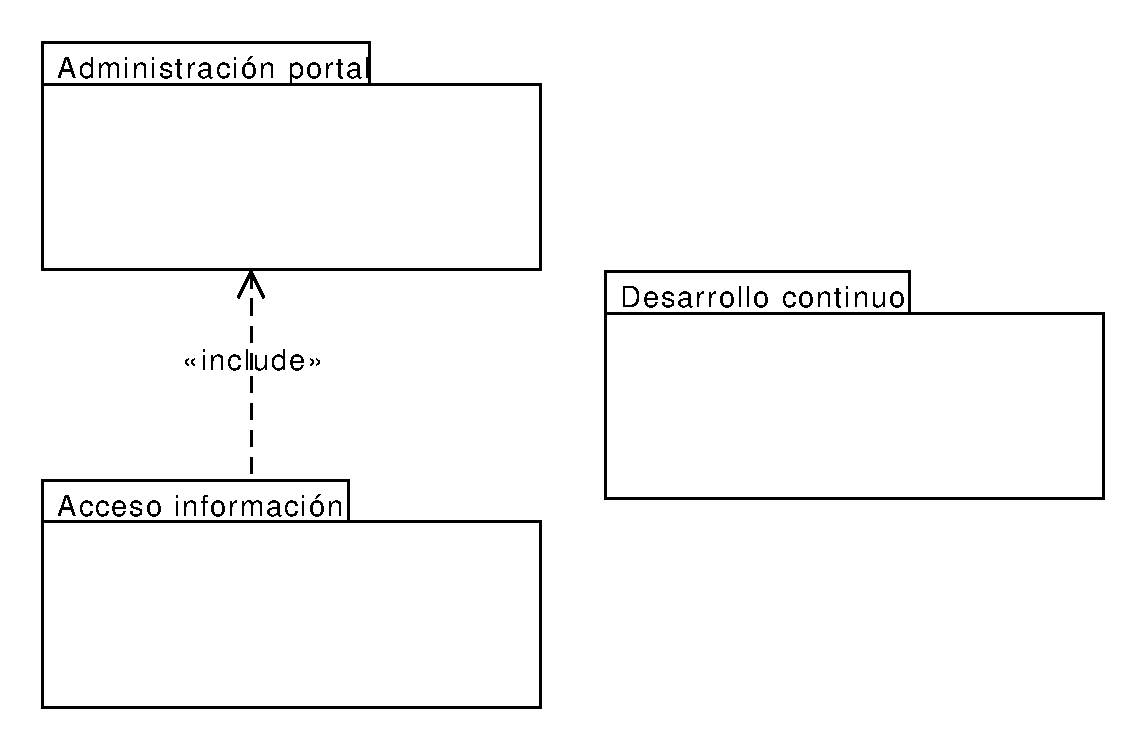
\includegraphics[width=0.8\textwidth]{../images/diagrama_paquetes.png}
  \caption{Diagrama de paquetes}
  \label{fig:diag_paquetes}
  \end{center}
\end{figure}
 
\section{Diagramas de casos de uso}

Los diagramas de casos de uso representa como los diferentes actores se relacionan con el sistema para usar sus funciones. Por ejemplo, en el primer caso de uso vemos como el \textbf{desarrollador} se relaciona con el sistema para iniciar el servidor del portal, mientras, en el segundo vemos como el \textbf{usuario} se relaciona con el sistema para consultar la información de las diferentes secciones del portal.

\begin{figure}[!ht]
  \begin{center}
  \includegraphics[width=0.65\textwidth]{../images/diag_cu_ap.png}
  \caption{Diagrama de casos de uso: paquete Administración portal}
  \label{fig:diag_cu_ap}
  \end{center}
\end{figure}

\begin{figure}[!ht]
  \begin{center}
  \includegraphics[width=0.65\textwidth]{../images/diag_cu_ai.png}
  \caption{Diagrama de casos de uso: paquete Acceso información}
  \label{fig:diag_cu_ai}
  \end{center}
\end{figure}

\newpage
\
\newpage
En el tercer diagrama vemos como el \textbf{desarrollador} se relaciona con los procesos relacionadas con las pruebas (que a su vez son dependientes entre sí); y en el cuarto vemos como también el \textbf{desarrollador} se relaciona con el sistema para realizar las tareas de configuración automática, como son el despliegue automático y el provisionamiento.

\begin{figure}[!ht]
  \begin{center}
  \includegraphics[width=0.65\textwidth]{../images/diag_cu_ps.png}
  \caption{Diagrama de casos de uso: paquete Pruebas de software}
  \label{fig:diag_cu_ps}
  \end{center}
\end{figure}

\begin{figure}[!ht]
  \begin{center}
  \includegraphics[width=0.65\textwidth]{../images/diag_cu_ca.png}
  \caption{Diagrama de casos de uso: paquete Configuración automática}
  \label{fig:diag_cu_ca}
  \end{center}
\end{figure}

\newpage
\section{Diagramas de actividad}

Los diagramas de actividad sirven para representar la descomposición de un proceso en las diferentes acciones de las que está compuesto. Las actividades de consultar algún tipo de información son procedimiento secuenciales en los que la ejecución es bastante simple; pero la actividad de iniciar el servidor del portal, realizar los test unitarios, realizar los test de cobertura, usar la integración continua tienen situaciones condicionales que son los que dan lugar a cursos alternos de la ejecución. Las actividades de despliegue automático y provisionamiento además tienen también puntos de sincronización que harán que el proceso siga el mismo cauce en su ejecución.

\begin{figure}[!ht]
  \begin{center}
  \includegraphics[width=1\textwidth]{../images/diag_act_cu_01.png}
  \caption{Diagrama de actividad CU-1. Inicio automático del servidor del portal}
  \label{fig:diag_act_cu_01}
  \end{center}
\end{figure}

\begin{figure}[!ht]
  \begin{center}
  \includegraphics[width=1\textwidth]{../images/diag_act_cu_02.png}
  \caption{Diagrama de actividad CU-2. Consultar información de Administración}
  \label{fig:diag_act_cu_02}
  \end{center}
\end{figure}

\begin{figure}[!ht]
  \begin{center}
  \includegraphics[width=1\textwidth]{../images/diag_act_cu_03.png}
  \caption{Diagrama de actividad CU-3. Consultar información de Docencia}
  \label{fig:diag_act_cu_03}
  \end{center}
\end{figure}

\begin{figure}[!ht]
  \begin{center}
  \includegraphics[width=1\textwidth]{../images/diag_act_cu_04.png}
  \caption{Diagrama de actividad CU-4. Consultar información de Gestión e Investigación}
  \label{fig:diag_act_cu_04}
  \end{center}
\end{figure}

\begin{figure}[!ht]
  \begin{center}
  \includegraphics[width=1\textwidth]{../images/diag_act_cu_05.png}
  \caption{Diagrama de actividad CU-5. Consultar información de Normativa Legal}
  \label{fig:diag_act_cu_05}
  \end{center}
\end{figure}

\begin{figure}[!ht]
  \begin{center}
  \includegraphics[width=1\textwidth]{../images/diag_act_cu_06.png}
  \caption{Diagrama de actividad CU-6. Realizar tests unitarios}
  \label{fig:diag_act_cu_06}
  \end{center}
\end{figure}

\begin{figure}[!ht]
  \begin{center}
  \includegraphics[width=1\textwidth]{../images/diag_act_cu_07.png}
  \caption{Diagrama de actividad CU-7. Realizar test de cobertura}
  \label{fig:diag_act_cu_07}
  \end{center}
\end{figure}

\begin{figure}[!ht]
  \begin{center}
  \includegraphics[width=1\textwidth]{../images/diag_act_cu_08.png}
  \caption{Diagrama de actividad CU-8. Usar integración continua}
  \label{fig:diag_act_cu_08}
  \end{center}
\end{figure}

\begin{figure}[!ht]
  \begin{center}
  \includegraphics[width=1\textwidth]{../images/diag_act_cu_09.png}
  \caption{Diagrama de actividad CU-9. Usar despliegue automático}
  \label{fig:diag_act_cu_09}
  \end{center}
\end{figure}

\begin{figure}[!ht]
  \begin{center}
  \includegraphics[width=1\textwidth]{../images/diag_act_cu_10.png}
  \caption{Diagrama de actividad CU-10. Usar provisionamiento}
  \label{fig:diag_act_cu_10}
  \end{center}
\end{figure}

\newpage
\
\newpage
\
\newpage
\
\newpage
\
\newpage
\
\newpage
\
\newpage
\
\newpage
\
\newpage

\section{Diagrama conceptual}

En el diagrama conceptual podemos ver una representación de la estructura de la implementación. A excepción de la clase \textbf{test}, todas las clases son parte de la aplicación principal (\textbf{app}) por lo que tienen una relación de composición con la misma y no tienen sentido sin esta. Las clases de \textbf{test} y \textbf{app} tiene una relación de agrupación, porque el módulo test puede realizar las pruebas sobre cualquier módulo de aplicación que sea recibido.

\begin{figure}[!ht]
  \begin{center}
  \includegraphics[width=1\textwidth]{../images/diagrama_conceptual.png}
  \caption{Diagrama conceptual}
  \label{fig:diagrama_conceptual}
  \end{center}
\end{figure}

\section{Otros diagramas o interfaces}

Gran parte de la implementación no va a ser de la aplicación principal en si misma, sino herramientas que se le van a agregar para obtener diferentes funcionalidades que se usarán durante su desarrollo, de ahí que no se considere necesario el realizar diagramas de comunicación ni diagramas de secuencia.

\bigskip
En cuanto a la interfaz gráfica, no será necesaria porque todas las herramientas solo tienen modo de funcionamiento a través de terminal.
%
%\chapter{Diseño}

\section{Diseño general del portal}

Para describir el diseño que se va a seguir en la programación del proyecto hay que tener en cuenta que se va a usar 
{\tt Node.js}, que está basado en el lenguaje de programación {\tt JavaScript} (que es un lenguaje orientado a objetos). Se 
usará un paradigma de programación orientado a objetos con diversas clases, que en este entorno de programación suelen ser 
referidos como módulos.

\bigskip
Existirá un módulo principal de la plataforma ({\tt app.js}) que será la plataforma en si misma, que es el encargado
de generar el servidor al que se realizarán las peticiones y visualizar cada unas de las páginas. Existirán también un módulo
por cada una de las secciones del portal: Administración ({\tt administración.js}), Docencia ({\tt docencia.js}), Gestión
e Investigación ({\tt gestionInvestigación.js}) y Normativa Legal ({\tt normativaLegal.js}. Si comparamos este esquema
con el de una aplicación más tradicional, podríamos considerar el módulo ({\tt app.js}) como la clase principal y el resto
de módulos como otras clases que tienen como función ser atributos compuestos de esa clase principal.

\bigskip
Cada uno de estos módulos de las diversas secciones, obtendrá la información para generar las páginas de sus subsecciones 
desde un archivo de datos {\tt JSON}, organizados de la siguiente forma.

\newpage
\begin{itemize}
 \item Portal de Transparencia ({\tt app.js})
 \begin{itemize}
  \item Administración ({\tt administración.js})
  \begin{itemize}
   \item Personal ({\tt personal.json})
   \item Información Económica ({\tt infoEcononica.json})
   \item Servicios ({\tt servicios.json})
  \end{itemize}
  \item Docencia
  \begin{itemize}
   \item Oferta y Demanda Académica ({\tt ofertaDemanda.json})
   \item Claustro ({\tt claustro.json})
   \item Estudiantes ({\tt estudiantes.json})
  \end{itemize}
  \item Gestión e Investigación
  \begin{itemize}
   \item Misión ({\tt mision.json})
   \item Plan Estratégico ({\tt .json})
   \item Gobierno ({\tt gobierno.json})
   \item Estadísticas ({\tt estadistica.json})
  \end{itemize}
  \item Normativa Legal
  \begin{itemize}
   \item Normativa Legal ({\tt normativaLegal.json})
  \end{itemize}
 \end{itemize}
\end{itemize}

Cada vez que un usuario quiere consultar la información de una subsección, el Portal de Transparencia hace una llamada al método
de generación de la página de la sección elegida para su subsección determinada; ese método, procesará la plantilla {\tt Jade}
para la página pasándole el archivo {\tt JSON} de datos y el resultado final será la página web que será visible en el portal.

\bigskip
De igual forma a lo mencionado de la aplicación del portal de transparencia, los test unitarios ({\tt test.js}) y el 
despliegue automático ({\tt flightplan.js}) son otros módulos que ejecutan dichas acciones, el test de cobertura se realiza
automáticamente a partir de los test unitarios, la integración continua se realiza en base a la configuración del archivo 
{\tt .travis.yml}, y finalmente, el aprovisionamiento sigue las tareas en el archivo de configuración {\tt transparente.yml}. 
Todos estos módulos son independientes del funcionamiento del módulo principal, y simplemente llamaremos cuando queramos hacer 
uso de sus funcionalidades.

\newpage
\section{Diseño de una aplicación con desarrollo colaborativo}

En varias ocasiones se ha indicado que este proyecto parte de un desarrollo colaborativo, esto es debido a que hoy en día es muy
dificil concebir un proyecto de software libre fuera de un entorno colaborativo que permita publicar el código libremente en
Internet donde sea accesible por cualquier persona, esta filosofía es la que sigue por ejemplo el desarrollo de {\tt Linux}
a principio de los años 90, el que se podría considerar como el más grande y relevante proyecto de software libre a nivel 
mundial. Además de abogar por la transparencia, este sistema de desarrollo hace que se más fácil encontrar errores durante el 
desarrollo ya que un mayor número de personas tienen acceso total al mismo. También hay que tener en cuenta como en todo 
proyecto que es imprescindible una herramienta de control de versiones, aún más en uno colaborativo donde es fácil que se 
produzcan conflictos en los archivos modificados por unos y otros desarrolladores.

\bigskip
La plataforma de desarrollo colaborativo y la herramienta de control de versiones a usar son {\tt GitHub} y {\tt Git} 
respectivamente. {\tt GitHub} es una de las plataformas de desarrollo colaborativo más usadas en proyectos libres y usa 
{\tt Git} como sistema de control de versiones para gestionar los proyectos que se almacenan en la plataforma. Estás son las 
herramientas que nos van a permitir que nuestro proyecto se convierta en un proyecto que se desarrollo de forma ágil, 
concretamente se va a seguir una metodología \textbf{DevOps}.

\bigskip
Una metodología de desarrollo \textbf{DevOps} consiste inicialmente en no hacer distinción entre el desarrollo del software y la
administración del mismo, todo estará comunicado para que sea posible realizar entregas del software de forma frecuente 
asegurándose de que esas mismas entregas continuas no sea el origen de fallos futuros. La forma de asegurarse de que esos
fallos no se producirán es dividir todo el desarrollo en fases que tengan que realizarse secuencialmente, controlando a cada
fase que no se produzcan errores en la misma; como una cadena de montaje en la que podemos estar seguro de que el producto
que llega al final está en perfectas condiciones, porque en caso contrario hubiera sido retirado durante el proceso.

\bigskip
En este proyecto, hemos considerado que las fases que nos permitirían asegurarnos que el producto que sale de la cadena de 
montaje en perfectas condiciones sean los test unitarios, la integración continua y el despliegue automático, todo esto apoyado
en un sistema de control de versiones y una plataforma de desarrollo colaborativo abierto. Además, también se usará
aprovisionamiento para facilitar la portabilidad del portal de una infraestructura a otra distinta. 

\section{Diseño de los tests unitarios y test de cobertura}

Para cumplir la parte de testeo de la implementación de la metodología DevOps, a partir del desarrollo de este proyecto se 
pretende seguir un desarrollo guiado por pruebas (en inglés, Test-Driven Development o TDD). Esto consiste en escribir primero
las pruebas que consideremos que la aplicación debe superar y luego desarrollar el código que realice la función que queremos
cumplir, pero superando dichas pruebas. 

\bigskip
Estas pruebas estarán basadas en la ejecución de tests unitarios que estarán diseñados para comprobar de forma de automática
que el código escrito cumple con el objetivo determinado; por lo que si una vez ejecutamos todos los tests unitarios, si no
obtenemos que todos han tenido una ejecución exitosa, tenemos que revisar el código escrito para saber por qué fallan.

\bigskip
Haciendo esto nos aseguraremos que todos las funcionalidades que vayamos añadiendo a la implementación de la aplicación
funcionarán correctamente; también nos asegura que si tenemos que hacer grandes modificaciones en el código, siempre que estas
modificaciones sigan pasando las pruebas, no deberemos preocuparnos por estropear el funcionamiento de la aplicación.

\bigskip
El tipo de test unitario que vamos a usar es un test basado en el comportamiento, es decir, la forma de evaluar si un test
se supera con éxito o fracaso es mediante la comprobación de la respuesta que da nuestra aplicación ante una solicitud 
determinada. Ejemplos:

\begin{itemize}
 \item Para comprobar que un archivo con datos de configuración ha sido cargado, el archivo cargado no debe ser nulo.
 \item Para comprobar que en la información cargado se encuentra el nombre de la categoria, la categoria debe tener una 
 propiedad llamada ``nombre''.
 \item Para comprobar que las páginas del portal están accesibles, las respuesta a las solicitudes se espera que tenga el valor
 200 (código de respuesta estándar para peticiones correctas en conexiones HTTP).
\end{itemize}

Pero el diseño de las pruebas no termina con escribir los tests unitarios que consideremos oportunos, también es necesario que
esos tests pasen a su vez un test de cobertura. Un test de cobertura comprueba el porcentaje de código desarrollado y/o
número de funciones de la aplicación que se están evaluando con los tests unitarios desarrollados, con esto se puede verificar
la completitud de los tests unitarios; si todos nuestros tests unitarios se evaluan correctamente, pero solo están cubriendo
un 30\% del total de la aplicación, este resultado satisfatorio no nos puede asegurar que la funcionalidad completa de la 
aplicación se vaya a ejecutar sin problemas.

\bigskip
Los tests unitarios se van a desarrollar usando Should y Supertest, ambos módulos de Node.js para evaluar comportamientos en las
peticiones. Estos tests unitarios a su vez van a ser evaluados por Mocha, un framework de JavaScript para testeo que se ejecuta
tanto en aplicaciones Node.js como en navegadores web. Por último, todo esto pasará por las pruebas de cobertura de código de 
Istanbul, que generará un informa detallado especificando la cantidad de código y el número de funciones que están cubiertas y
también los que no.

\section{Diseño de la integración continua}

\section{Diseño del despliegue automático}

\section{Diseño del aprovisionamiento}
%
%\chapter{Implementacion}
 
\section{Uso de JSON como origen de datos}
 
[Explicar el problema que motivó el cambio de usar una base de datos MongoDB a usar archivos JSON]

\begin{lstlisting}[language=json,caption={Archivo JSON con informacion de personal},label={lst:json_personal}]
{
  "nombre":"Personal",
  "plantilla":"personal",
  "contenido":[
    {
      "encabezado":"Informacion Salarial 2015",
      "link":"informacion-salarial-2015",
      "texto":"Informacion relativa a la oferta..."
    },
    
  ],
  "datos":[
    {
      "dataset":"Informacion Salarial 2015",
      "id_dataset":"informacion-salarial-2015",
      "nombre":"Analisis total plantilla: genero",
      "vista":1,
      "url":"51d53138-0408-4257-9909-57acea137a58",
      "descarga":"985a8e1e-734b-432a-ac65-a7da..."
    },
        
  ]
}
\end{lstlisting}

\begin{lstlisting}[language=javascript,caption={Archivo {\tt cargar.js}},label={lst:cargarjs}]
var fs = require("fs");
 
var cargar = function (archivo){
  var config = null;

  try{
    config = JSON.parse(fs.readFileSync(archivo));
  }
  catch(e){
    console.log("Error: no existe el archivo " + archivo);
  }

  return config;
};

module.exports = cargar;
\end{lstlisting}

\begin{lstlisting}[language=javascript,caption={Archivo {\tt app.js}},label={lst:appjs}]
var express = require('express');
var http = require('http');

var administracion = require(__dirname+'/routes/administracion');

var cargar = require(__dirname+'/lib/cargar');

module.exports.config = cargar(__dirname+'/config/config.json');
module.exports.personal = cargar(__dirname+'/config/personal.json');

app.get('/personal.html',administracion.personal);
app.get('/archivos/personal', function(req, res) {
  res.send(cargar(__dirname+'/config/personal.json'));
});

http.createServer(app).listen(app.get('port'), app.get('ip'), function(){
  console.log('Express server listening on ' + app.get('ip') + ':' + app.get('port'));
});

module.exports = app;
\end{lstlisting}

\begin{lstlisting}[language=javascript,caption={Archivo {\tt administracion.js}},label={lst:adminjs}]
var conf = require('../app');

exports.personal = function(req, res){
  var personal = conf.personal;

  res.render(personal.plantilla, {
    servidor: conf.config.servidor,
    seccion: personal.nombre,
    contenido: personal.contenido,
    datos: personal.datos,
  });
};
\end{lstlisting}

\begin{lstlisting}[language=json,caption={Scripts de inicio y detención},label={lst:ini_para}]
"scripts": {
  "start": "PORT=3000 IP=127.0.0.1 forever start -l /var/log/forever.log -a -o /var/log/out.log -e /var/log/err.log ./app.js",
  "kill": "ps aux | grep 'app.js' | grep -v grep | awk '{print \"sudo kill -9 \" $2}' | sh"
}
\end{lstlisting}

\section{Tests unitarios y de cobertura}

\begin{lstlisting}[language=javascript,caption={Archivo {\tt test.js}},label={lst:testjs}]
var should = require("should"),
request = require("supertest");

describe('Test de carga y formato de JSONs', function(){
  describe('Archivo de configuracion', function(){
    var config = cargar(__dirname+"/../config/config.json");

    describe('Carga de archivo', function(){
      it('Cargado', function(){
        config.should.not.be.null;
      });
    });

    describe('Formato de archivo', function(){
      describe('Campos obligatorios', function(){
        it('nombre', function(){
          config.should.have.property("nombre");
        });
      });
    });
    
  });
};

describe('Prueba de acceso', function(){
  _.each(acceso.elemento, function(valor) {
    it(valor.nombre, function(done){
      request(app)
      .get(valor.ruta)
      .expect(200)
      .end(function(err, res){
        if (err){
          throw err;
        }
        done();
      });
    });
  });
});
\end{lstlisting}

\begin{lstlisting}[language=json,caption={Scripts de test},label={lst:test}]
"scripts": {
  "test": "istanbul cover _mocha ./test --recursive"
}
\end{lstlisting}

\section{Integración continua}

\begin{lstlisting}[language=json,caption={Archivo JSON con informacion de personal},label={lst:json_personal}]
# language setting
language: node_js

# version numbers, testing against two versions of node
node_js:
- "0.12"
- "0.11"
- "0.10"
- "iojs"
\end{lstlisting}

\section{Despliegue automático}

\begin{lstlisting}[language=javascript,caption={Archivo {\tt test.js}},label={lst:testjs}]
var plan = require('flightplan');

plan.target('transparente', {
  host: 'transparente.ugr.es',
  username: process.env.USER,
  agent: process.env.SSH_AUTH_SOCK
});

plan.remote(function(remote) {
  remote.log('Creando copia de seguridad...');
  remote.sudo('cp -Rf ugr-transparente-servidor ugr-transparente-servidor.bak', {user: process.env.USER});

  remote.with('cd ugr-transparente-servidor',function() {
    remote.log('Deteniendo el servidor...');
    remote.exec('sudo npm run-script kill');
    remote.log('Restableciendo parametros de acceso...');
    remote.exec('sed "s/IP=transparente.ugr.es/IP=127.0.0.1/" -i package.json');
    remote.exec('sed "s/PORT=80/PORT=3000/" -i package.json');
    remote.log('Obteniendo cambios...');
    remote.exec('git pull');
    remote.log('Instalando dependencias...');
    remote.exec('sudo npm install');
    remote.log('Cambiando parametros de acceso...');
    remote.exec('sed "s/IP=127.0.0.1/IP=transparente.ugr.es/" -i package.json');
    remote.exec('sed "s/PORT=3000/PORT=80/" -i package.json');
    remote.log('Arrancando el servidor...');
    remote.exec('sudo npm start');
  });
});
\end{lstlisting}

\begin{lstlisting}[language=json,caption={Scripts de despliegue automático},label={lst:deploy}]
"scripts": {
  "deploy": "fly transparente"
}
\end{lstlisting}

\section{Aprovisionamiento}

\begin{lstlisting}[language=json,caption={Archivo de hosts},label={lst:hosts}]
[transparente]
transparente.ugr.es
\end{lstlisting}

\begin{lstlisting}[language=json,caption={{\tt Playbook} de {\tt Ansible}},label={lst:ansible}]
---
- hosts: transparente
  sudo: yes
  remote_user: "{{user}}"
  tasks:
    - name: Añadiendo repositorio para instalar Node.js...
      apt_repository: repo='ppa:chris-lea/node.js'

    - name: Actualizando lista de paquetes...
      apt: update_cache=yes

    - name: Instalando git...
      apt: name=git state=present

    - name: Instalando Node.js...
      apt: name=nodejs state=present

    - name: Clonando repositorio con la aplicacion...
      git: repo=https://github.com/oslugr/ugr-transparente-servidor.git
           dest=/home/"{{user}}"/ugr-transparente-servidor
           version=master

    - name: Cambiando propietario del directorio de la aplicacion...
      file: path=/home/"{{user}}"/ugr-transparente-servidor
            owner="{{user}}" group="{{user}}" state=directory recurse=yes

    - name: Instalando las dependencias de la aplicacion...
      npm: path=/home/"{{user}}"/ugr-transparente-servidor

    - name: Cambiando parametros de acceso (1/2)...
      command: sed "s/IP=127.0.0.1/IP=transparente.ugr.es/" -i
               /home/"{{user}}"/ugr-transparente-servidor/package.json

    - name: Cambiando parametros de acceso (2/2)...
      command: sed "s/PORT=3000/PORT=80/" -i
               /home/"{{user}}"/ugr-transparente-servidor/package.json

    - name: Arrancando el servidor...
      command: chdir=ugr-transparente-servidor npm start
\end{lstlisting}
%
%\chapter{Pruebas}

\section{Pruebas unitarias}

\begin{figure}[!ht]
	\begin{center}
		\includegraphics[width=1\textwidth]{../images/tests_unitarios_01.png}
		\caption{}
		\label{fig:tests_unitarios_01}
	\end{center}
\end{figure}

\begin{figure}[!ht]
	\begin{center}
		\includegraphics[width=1\textwidth]{../images/tests_unitarios_02.png}
		\caption{}
		\label{fig:tests_unitarios_02}
	\end{center}
\end{figure}

\section{Prueba de cobertura}

\begin{figure}[!ht]
	\begin{center}
		\includegraphics[width=1\textwidth]{../images/test_cobertura_01.png}
		\caption{}
		\label{fig:test_cobertura_01}
	\end{center}
\end{figure}

\begin{figure}[!ht]
	\begin{center}
		\includegraphics[width=1\textwidth]{../images/test_cobertura_02.png}
		\caption{}
		\label{fig:test_cobertura_02}
	\end{center}
\end{figure}

\begin{figure}[!ht]
	\begin{center}
		\includegraphics[width=1\textwidth]{../images/test_cobertura_03.png}
		\caption{}
		\label{fig:test_cobertura_03}
	\end{center}
\end{figure}

\section{Integración continua}

\begin{figure}[!ht]
	\begin{center}
		\includegraphics[width=1\textwidth]{../images/integracion_continua_01.png}
		\caption{}
		\label{fig:integracion_continua_01}
	\end{center}
\end{figure}

\begin{figure}[!ht]
	\begin{center}
		\includegraphics[width=1\textwidth]{../images/integracion_continua_02.png}
		\caption{}
		\label{fig:integracion_continua_02}
	\end{center}
\end{figure}

\begin{figure}[!ht]
	\begin{center}
		\includegraphics[width=1\textwidth]{../images/integracion_continua_03.png}
		\caption{}
		\label{fig:integracion_continua_03}
	\end{center}
\end{figure}

\newpage \
\newpage \
\newpage \
\newpage \
\newpage \
\section{Prueba de carga}

\subsection{Métricas y parámetros que afectan al rendimiento}

Para comparar las prestaciones de la aplicación debemos tener en cuenta los siguientes criterios:

\begin{itemize}
	\item El objetivo de esta prueba es medir las prestaciones del servidor generado por {\tt Express} para dar servicio a la aplicación del portal de transparencia bajo unas condiciones que nos aporte un análisis neutro del rendimiento del mismo.
	\item La herramienta que se usará para realizar estás mediciones es {\tt ApacheBench}.
	\item Los parámetros que se considerarán los parámetros usados en la herramienta: el número de peticiones que se realizan al servidor y el nivel de concurrencia con el que se realizan las peticiones.
	\item Los valores de estos parámetros irán modificándose para tener unos resultados más completos ante las diferentes cargas de trabajo que soportará el servidor.
\end{itemize}

El hardware y el software del sistema serán los siguientes:

\begin{itemize}
	\item \textbf{Hardware}:
	\begin{itemize}
		\item Procesador: Intel Pentium Dual CPU E2180 @ 2.00GHz
		\item Placa base: MSI MS-7255
		\item Chipset: VIA P4M900
		\item Memoria: 3GB (2+1 DIMM DDR2)
		\item Disco: Maxtor 6Y160P0 160GB 7200RPM
		\item Tarjeta gráfica: ATI Radeon X300SE 325MHz 128MB
		\item Red: Realtek RTL8100C 100Mbps
	\end{itemize}
	\item \textbf{Software}:
	\begin{itemize}
		\item Sistema operativo: Ubuntu 14.04.1 LTS i686 GNU/Linux
		\item Kernel: Linux 3.13.0-35-generic
		\item Sistema de archivos: ext4
	\end{itemize}
\end{itemize}

\subsection{Técnicas de evaluación, carga de trabajo y diseño de experimentos}

Para evaluar el rendimiento de la aplicación vamos a realizar benchmark hacia la aplicación en ejecución para poder realizar una evaluación sobre su comportamiento bajo diferentes cargas de trabajo. El programa con el que vamos hacer las pruebas es el ya mencionado {\tt ApacheBench}.
{\tt ApacheBench} es un aplicación en modo terminal que permite realizar de forma sencilla pruebas de rendimiento a cualquier servidor, sea cual sea el lenguaje en el que esté realizado. 

\bigskip
Según la información de registros de acceso del servidor en los últimos \textbf{6 meses} el número de peticiones de páginas del portal ha sido de \textbf{2.388 peticiones}, lo que sería aproximadamente \textbf{13 peticiones/día}. Para realizar los diferentes tests se realizará un \textbf{número de conexiones} variables al servidor (\textbf{30, 50 y 100}) con diferentes \textbf{niveles de concurrencia} en función del total de conexiones (\textbf{25\%, 50\% y 75\%}). Los números de conexiones para las prueba han sido elegidos para evaluar como se comportaría el servidor ante un gran aumento de actividad en el mismo en línea con el nivel de conexiones que se producen en la actualidad.

\bigskip
De entre las peticiones al portal, la página que ha recibido un mayor número de peticiones es la página de \textbf{Personal}, por lo que se van a realizar dos experimentos: el primero consistirá en realizar únicamente peticiones de la página de \textbf{Personal} a la aplicación; el segundo consistirá en realizar peticiones a distintas páginas de la aplicación de forma aleatorio. Estos experimentos nos permitirán comprobar como se comportará la aplicación en diferentes situaciones cono diferentes nivele de carga y la repercusión en su rendimiento ante estás diferentes pruebas, viendo por ejemplo si fuera necesario buscar una forma de balancear la carga del servidor. 

\bigskip
En total cada experimento constará de 9 pruebas, y a su vez cada una de estas pruebas se repetirá 10 veces consecutivas para así asegurarnos que los resultados son legítimos y no producto de sucesos fortuitos.

\bigskip
Las variables respuestas a tener en cuenta para el estudio serán:

\begin{itemize}
	\item Tiempo de ejecución.
	\item Solicitudes por segundo.
	\item Tiempo por solicitud concurrente.
	\item Velocidad de transferencia.
\end{itemize}

\bigskip
El único factor para los experimentos serán, como hemos dicho, el servidor de la aplicación desarrollada del portal de transparencia {\tt UGR Transparente}. Cuando se disponga de los resultados de todas las pruebas, se procederá a analizar e interpretar los resultados.

\subsection{Presentación de los resultados}

Enumeración de las pruebas a realizar por cada experimento:

\begin{itemize}
	\item \textbf{P1}: 30 solicitudes, concurrencia del 25\% (8).
	\item \textbf{P2}: 30 solicitudes, concurrencia del 50\% (15).
	\item \textbf{P3}: 30 solicitudes, concurrencia del 75\% (23).
	\item \textbf{P4}: 50 solicitudes, concurrencia del 25\% (13).
	\item \textbf{P5}: 50 solicitudes, concurrencia del 50\% (25).
	\item \textbf{P6}: 50 solicitudes, concurrencia del 75\% (38).
	\item \textbf{P7}: 100 solicitudes, concurrencia del 25\% (25).
	\item \textbf{P8}: 100 solicitudes, concurrencia del 50\% (50).
	\item \textbf{P9}: 100 solicitudes, concurrencia del 75\% (75).
\end{itemize}

\subsubsection{Experimento 1: peticiones a Personal}

\begin{itemize}
	\item \textbf{Tiempo de ejecución}
	\item \textbf{Solicitudes por segundo}
	\item \textbf{Tiempo por solicitud concurrente}
	\item \textbf{Velocidad de transparencia}
\end{itemize}
%
%\chapter{Conclusiones y trabajos futuros}

Después de realizar este proyecto la principal conclusión a la que se puede llegar es que si bien un desarrollado menos \textit{instrumentado} puede ser muy rápido, el dividir el desarrollo en diferentes etapas (con herramientas que a su vez tienen sus propios sistemas de control) harán del desarrollo una tarea más fácil y robusta.

\bigskip
Este era uno de los principales problemas del estado inicial del portal, al no encontrarse por ejemplo implementados ningún tipo de tests unitarios se producían varios errores por causas desconocidas que eran difíciles de situar en el código de la aplicación.

\bigskip
Uno de los principales problemas, es que para esta metodología de desarrollo las fases de planificación y análisis pueden ser más difíciles de plantear, ya que se basa en un desarrollo continuo en el que todo elemento a desarrollar se decide según la necesidad y generalmente con un tiempo de antelación bastante corto.

\bigskip
Como ventaja tenemos que hay un gran cantidad de herramientas para gestionar las diferentes etapas, pudiendo elegir las que consideremos precisas en un determinado momento ya sea por restricciones del desarrollo o por simple comodidad. Por ejemplo: los test unitarios se podrían haber pasado con {\tt Unit JS}, la integración continua con {\tt Jenkins} y el provisionamiento con {\tt Chef}; así aunque los procedimientos fueran distintos, el resultado hubiera sido el mismo.

\newpage
En cuanto a trabajos futuros relacionados con el proyecto algunas posibilidades serían:

\begin{itemize}
	\item Realizar un instalación personalizada de {\tt CKAN} en un versión actual de {\tt Ubuntu} (actualmente solo existe una instalación oficial para la versión 12.04) para poder desarrollar
	plugins propios con el fin de realizar tareas que se puedan considerar interesantes; principalmente interesa que los datos se pudieran obtener directamente desde el propio {\tt CKAN} y no se tuvieran que introducir manualmente mediante archivos \textit{JSON}. Este era uno de los objetivos del proyecto, pero por su dificultad para realizarlo en el periodo de tiempo establecido se determinó que fuera un objetivo secundario; finalmente no ha podido ser cumplido por dicho motivo, por lo que queda como una posible extensión del trabajo inicial.
	\item Sería conveniente hacer que en general que el portal sea más dinámico porque actualmente todas las páginas son estáticas, si eso se mantiene así en unos cuantos años cuando la cantidad de datos disponibles aumente considerablemente, la navegabilidad por el portal empeorará considerablemente. Sería necesario implementar un forma de que se puedan seleccionar para visualizar solo los datos que se deseen.
	\item Analizando los resultados de las pruebas de carga observamos que cuando el número de peticiones aumentaba en gran cantidad con respecto a la carga de trabajo actual, o aunque las peticiones no aumentaran tanto, pero si aumentase el nivel de concurrencia la aplicación se saturaba. Estoy debería ser solucionado mediante cambios en las estructura de la aplicación o uso de balanceo de carga.
\end{itemize}
%
%%\chapter{Conclusiones y Trabajos Futuros}
%
%%\nocite{*}
%\bibliography{bibliografia/bibliografia}\addcontentsline{toc}{chapter}{Bibliografía}
%\bibliographystyle{miunsrturl}
%
%\appendix
%\input{apendices/manual_usuario/manual_usuario}
%\input{glosario/entradas_glosario}
%\addcontentsline{toc}{chapter}{Glosario}
%\printglossary

\thispagestyle{empty}

\end{document}
